\chapter{科学道德与学风}

学位论文撰写时要遵循科学道德,树立良好学风。本章介绍科学道德与学风中和学位论文撰写密切相关的四个方面,在撰写学位论文时要拒绝科研不端行为,规避科研不当行为,注意科研规范和引文规范。\textcolor{red}{(注:仅参考此格式进行排版。)}

\section{科学道德与学风问题}

科学道德与学风问题是指科技工作者在科研规范、行为准则、治学精神、治学态度、治学风气、治学原则等方面出现的失范现象。反映了现代科研体制在科研活动中存在的问题和漏洞,既有科技工作者精神层面的伦理道德问题,也有行为层面的科研规范问题[3]。

中国科协《科技工作者科学道德规范(试行)》规定的违反科学道德的学术不端行为主要表现为七种类型,具体描述见附录B。

\section{科研不端行为}

本节内容均摘自文献[3],后文未一一引用。

\subsection{科研不端行为的定义}

国际科技界将严重违反基本的科学诚信的行为称为科研不端行为(misconduct in science,或称scientific misconduct),这种行为与科研违规行为、科研越轨行为的内涵十分接近。科研不端行为主要有以下三方面特征:第一,违反科学界通用的道德标准,或严重背离相关研究领域的行为规范;第二,不端行为是蓄意的、明知故犯的或是肆无忌惮的;第三,不端行为不包括诚实的错误或者观点的分歧。

综上所述,科研不端行为的理解如图5.1所示。

2007年,中国科学院发布《中国科学院关于加强科研行为规范建设的意见》,明确将科研不端行为进行定义,并分为以下几类:

1)在研究和学术领域内有意做出虚假的陈述,包括:编造数据;篡改数据;改动原始文字记录和图片;在项目申请、成果申报,以及职位申请中做虚假的陈述。

\begin{figure}[htbp]
	\centering
	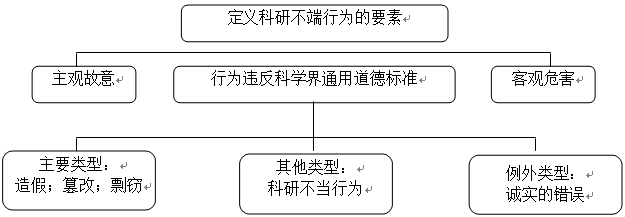
\includegraphics[width=12cm]{images/chapters/5.1}
	\caption{科研不端行为的理解} 
	\label{fig:5.1} 
\end{figure}

2)损害他人著作权,包括:侵犯他人的署名权,如将做出创造性贡献的人排除在作者名单之外,未经本人同意将其列入作者名单,将不应享有署名权的人列入作者名单,无理要求著者或合著者身份或排名,或未经原作者允许用其他手段取得他人作品的著者或合著者身份。剽窃他人的学术成果,如将他人材料上的文字或概念作为自己的发表,故意省略引用他人成果的事实,使人产生为其新发现、新发明的印象,或引用时故意篡改内容、断章取义。

3)违反职业道德利用他人重要的学术认识、假设、学说或者研究计划,包括:未经许可利用同行评议或其它方式获得的上述信息;未经授权就将上述信息发表或者透露给第三者;窃取他人的研究计划和学术思想据为己有。

4)研究成果发表或出版中的科学不端行为,包括:将同一研究成果提交多个出版机构出版或提交多个出版物发表;将本质上相同的研究成果改头换面发表;将基于同样的数据集或数据子集的研究成果以多篇作品出版或发表,除非各作品间有密切的承继关系。

5)故意干扰或妨碍他人的研究活动,包括故意损坏、强占或扣压他人研究活动中必需的仪器设备、文献资料、数据、软件或其他与科研有关的物品。

6)在科研活动过程中违背社会道德,包括骗取经费、装备和其他支持条件等科研资源;滥用科研资源,用科研资源谋取不当利益,严重浪费科研资源;在个人履历表、资助申请表、职位申请表,以及公开声明中故意包含不准确或会引起误解的信息,故意隐瞒重要信息。

\subsection{科研不端行为的表现形式}

从表现形式看,有三类科研不端行为,即杜撰、篡改、剽窃(FFP)。

\textbf{1)杜撰(fabrication)}

杜撰一般指按照某种科学假说和理论演绎出的期望值伪造虚假的观察与实验结果,从而支持理论的正确性或者确认实验结果的正确性。它表现为对科学和实验结果的不尊重,按照个人主观意愿无中生有,捏造事实。

按照科研的内容和程序分类,杜撰主要分两种:第一,科研申请中的杜撰。主要指在项目资金申请、科研成果申报,以及职位申请等其他科研活动中做虚假的陈述,如杜撰学历、杜撰论文或书刊发表记录、提供虚假获奖证书、文献引用证明,等等;第二,科研过程中的杜撰。主要指在科研过程中,未经过试验、调查,仅根据局部科学现象甚至根本没有根据,凭空编造、虚拟出一些试验数据、结果或事实、证据来作为支持自己论点的论据,证明某理论的正确性。而凭空编造出来的数据或实验结果不具有可重复性,与真实的数据互不兼容。

\textbf{2)篡改(falsification)}

篡改,主要是指在科研过程中,用作伪的手段按自己的期望随意改动、任意取舍原始数据或试验使得结果符合自己的研究结论、支持自己的论点。

篡改数据违背了科研规范中的一个基本要求,就是要忠实的记录和保存原始数据。用个人主观意愿对科研结果横加干预,其实验结果必然不具有可重复性。

篡改行为的表现形式主要包括两种:第一,篡改数据,主要指以一些实验结果为基础推测实验结果,对另一些与推测其他结果不同的实验结果、实验记录和图片进行修改。第二,拼凑数据,主要指按期望值主观取舍、任意组合实验结果,或者把与期望值不符的实验结果删除,只保留与期望值一致的实验结果。

\textbf{3)剽窃((plagiarism)}

剽窃是指将他人的科研成果或论文全部或部分原样照抄,并以自己名义发表的欺诈行为。它不仅包括对他人作品字句、内容的直接使用,也包括对他人学术论著的思想、观点、结构、体系等元素作为自己论著的基本元素加以使用并发表的行为。通常表现为不尊重他人学术思想、学术观点,不注明学术思想、学术观点的出处来源而随意使用。

在学术研究中,对已有成果的了解是必需的,对已有成果的借鉴也是不可避免的,因此是否适当引用就成为判断剽窃或借鉴的关键。正确的引用包括两个方面的含义:一是凡借鉴就要引用,引用就要对原出处进行明示;二是引用只能反映研究者对本研究领域已有研究成果的了解和借鉴,或反映已有成果与自己研究的关系,不能构成自己研究成果的主体内容。

\section{科研不当行为}

本节内容均摘自文献[3]。

\subsection{科研不当行为的定义}

科研不当行为(questionable research practice,QRP)是指虽然违反科学的目的、精神和科学研究事业的基本道德原则,但没有直接触犯明确规定的研究活动的道德底线的行为。

科研不当行为的特征主要为:第一,科研不当行为以明确不违反科学共同体规约为前提,更不是一种违法行为。第二,科研不当行为虽然不是科学共同体规约所明确禁止,但它是不合理的,具有不合理、不公正、不合乎科学道德的特征。

\subsection{科研不当行为的表现形式}

科研不当行为的表现形式很多,一般来说,科研不当行为主要可分为五种类型:

\textbf{1)数据的不当使用}

(1) 根据本能感觉,排除本人认为不精确的观测或数据点;或因匆忙完成项目而偷工减料;

(2)未能在合理的期间内获得重要研究数据;

(3)维持不充分的研究记录,特别是那些用于发表或被他人所依赖的结果;

(4)运用不恰当的统计学或其他计量方法提高研究结论的重要性;

(5)在论文中给出理由的情况下将异常值从数据集中剔除;

(6)为了提高研究的重要性,运用不恰当的统计方法;

(7)窃取供应品、书籍或数据;

(8)操纵实验以获得本人想要的结果;

(9)未经许可复制数据、论文或软件程序;

(10)在合理的期间内,未能保持良好的研究记录或研究数据。

\textbf{2)违反科学规则}

(1)忽视材料处理政策的细节(如生物安全、放射性材料等);运用一个项目的资金完成其他项目;

(2)在人体研究实验中没有报告不良事件;

(3)在研究中不珍惜动物资源;

(4)违反本人所在研究机构的生物安全规定而未尽告知义务,将员工和学生暴露于生物风险之中。

\textbf{3)不当的同行关系则}

(1)通过与论文研究无重要关联的特殊服务获取署名;

(2)在同事没有对论文作出重大贡献的情况下将其列为作者,以作为人情回报;

(3)为了确保本人成为唯一的发明人,未告知合作者本人申请专利的意图;

(4)未经授权运用他人的想法,或对这种使用未给予应有的感谢;

(5)与同事讨论本人所正在承担的期刊论文审稿工作中获得的保密数据;

(6)规避同行审查程序并通过媒体发布会公布本人的研究结果,而未给予同行足够的时间评估本人的工作;

(7)在文献综述中未能表明在该领域的其他人或相关前期工作的贡献;

(8)妨害他人的工作;

(9)评审他人论文时未经认真阅读即拒绝论文的发表;

(10)在评审工作中做出贬损的评论乃至贬损他人人格;

(11)拒绝同行接触作为已发表论文之支撑的独一无二的研究材料或数据。

\textbf{4)不当的师生关系}

(1)基于财、物、性等交易行为许诺学生以更好的成绩;

(2)过度使用、忽略或剥削研究生或博士后的劳动;

(3)提供过于正面或过于负面的推荐信。

\textbf{5)基于产出压力的不当科研}

(1)在基金项目的申请中夸大事实,以说服评审人此项目将会对该领域做出重大贡献;

(2)为了应对资助方的压力,修改研究的设计、方法或者结果;

(3)在论文或计划中保留方法或结果的细节;

(4)将推测歪曲为事实或者公布初步的研究结果(特别是在大众媒体上),而未能提供充分的数据使得同行可以评判结果的有效性或重复该实验;

(5)在两种或两种以上不同的期刊上发表相同的论文,而未告知编辑,即一稿多投或一稿多发;

(6)在工作申请或建立中夸大事实;

(7)在资助本人研究的公司中拥有实质性数量的股份而未披露此种经济利益;

(8)故意夸大新药的临床效果以获得经济利益。

\section{科研规范}

本节内容均摘自文献[3]。

科研规范(或学术规范)主要是指从事科研活动的行为规范,是以科研道德为基础,以科学共同体为主体,对科研及其相关行为作出的规制性安排。当代科技工作者应坚持的科研规范包括:诚实原则、公开原则、公正原则、尊重知识产权、声明与回避原则。

\subsection{研究数据收集、记录和保存中的规范}

数据直接影响到研究成果,因此应当从源头上抓好数据的规范行为。

在数据收集过程中,首先应保证获得数据的条件是真实的,而不是虚构的;其次要确保收集和保存实验数据的完整性;第三,不能为某种目的或获取利益对原始数据进行人为加工和篡改;第四,收集特殊数据应当事先获得授权许可。

数据记录应当与数据的获得同步。数据记录必须精准,必须严格按照有关程序和规则记录数据。

在数据保存方面,第一,应以严谨的方式保存数据。如果是书面记录,就要存放在安全的地方;如果是计算机文件,就应备份,并注意将备份的数据保存在安全处,备份数据应与原始数据分开保存,并且定期为所保存的数据重新备份。第二,原始数据应由产生这些数据的研究机构和科研人员共同保存。第三,要慎重保存涉及机密或危险的数据。第四,应做好数据保存相关事项的预先协议。第五,遵守数据保存期限但不应有意隐蔽数据。

\subsection{研究数据使用中的规范}
在未通过发表物或公开宣布研究成果而确立优先权之前,科研人员可以独自使用已经得到确证或有效的数据。一旦科研人员将实验结果公开发表,其他人就可以自由地获取实验涉及到的所有数据,包括最终结果,以便于检验和使用。

在数据使用和处理成图像过程中,首先,应当保证原始数据的真实性,并且保证图像是对数据的真实体现;其次,论著中的数据图像必须是原始记录的完整体现;第三,他人制作完成的数据图像应当在论著中予以说明;第四,应当熟知和合理运用现有相关处理数据的计量方法;第五,应当预先了解拟投稿的相关出版社或期刊的数据和图像处理规范或相关指南;第六,应当了解哪些行为是会受到处罚,以及将会受到怎样的处理。


\subsection{引文的规范}
引文的规范可参考中国国家标准局2005年发布并实施的《文后参考文献著录规则》。通常已经发表的论著或文章可以不经作者授权就自行引用,对于未正式发表的资料,未经所有者的许可,不应随意引用。

引用时需要避免的七种行为:

\textbf{1)著而不引。}

一些作者把原作者的研究进行改头换面,再用自己的语言叙述出来,并当作自己的论述而不注明出处。这种行为虽然在表达上可能是作者自己的话,实际上,作者只是挪用了别人的观点、想法或理念,并不是作者自己的研究,所以是一种剽窃行为。

\textbf{2)引而不著。}

利用引注或者改写/转述引文,并以之构成自己论著作的主要部分或核心内容,即为引而不著。这种对引注的不恰当或过度使用,也是一种剽窃行为。

\textbf{3)有意漏引。}

在引用文献综述特定领域的研究、或者佐证自己的研究时,应当公正地涵盖已有的研究,如果为了减少工作量而故意不去查阅一部分文献,或者只选择对自己研究有利的研究,或者为了突出自己研究的意义而不提及某些已有研究,等等,均为有意漏引。这是一种欺骗行为。

\textbf{4)过度他引。}

引文应当是作者在撰写论著时确实参考或引用过的文献,如果为了给人一种阅读了大量文献资料、研究基础扎实的印象,而故意在论著中加入大量实际没有参考或引用过的、或者与本文论题根本不相干的文献,做不相关引用、无效引用,就是过度他引了。这是一种伪注。

\textbf{5)不当自引。}

作者撰写论著时,出于提高引用率,或扩大影响等目的,不必引而偏引,进行不必要的过度自我引用。这是一种欺骗行为。

\textbf{6)相互引用。}

引用应当完全出于学术目的,但有一些作者为了提高彼此的引用率,采取“团体作战”的方式,在小团体之间进行,以提高彼此引用率为目的的相互引用。这样做即使提高了引用率,也是圈内相互消化的结果,并不体现真实的引用率和论文质量。这是一种作假和欺骗行为。
\newpage %将下面内容放在新一页,使得排版美观
\textbf{7)模糊引注。}

为逃避被指责为抄袭的可能,一些论著在直接引用了他人的相关文献后,并不标出具体的引文出处,如分册数、页码等,而将它们笼统地放在文后参考文献,从而给人从总体上只是参考了某一文献的印象。

\section{本章小结}
介绍了科研不端行为和科研不当行为以及科研规范。










